\section{Normalization} \label{sec:L2_Normalization}

\blindtext
\autocite{pedregosa_scikit-learn_2011}

\blindtext

\begin{figure}
    \centering
    %\begin{adjustbox}{minipage=\dimexpr\textwidth-2\fboxsep-2\fboxrule,fbox}
    \begin{subfigure}[b]{0.475\textwidth}
        \caption[Dimension Reduction with \Acrshort{PCA}]{\textbf{Dimension Reduction with \Acrshort{PCA}}}
        \label{subfig:Normalisation_PCA}            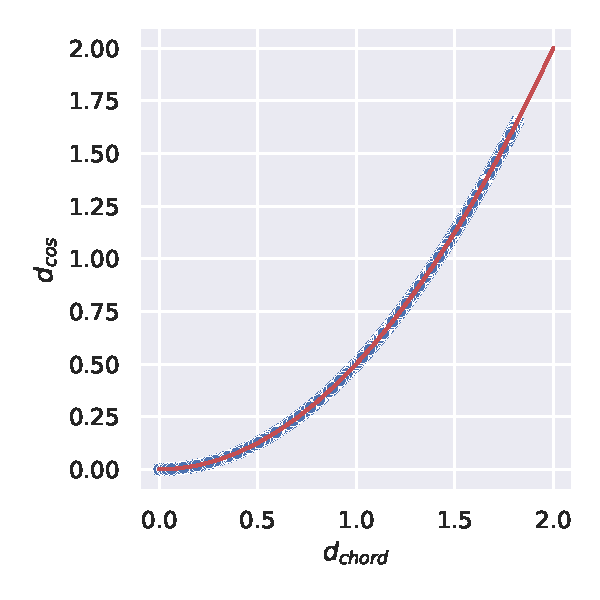
\includegraphics[width=\textwidth]{PCA/Difference_Distance_Calculation.pdf}
    \end{subfigure}
    \hfill
    \begin{subfigure}[b]{0.475\textwidth}
        \caption[Dimension Reduction with \Acrshort{UMAP}]{\textbf{Dimension Reduction with \Acrshort{UMAP}}}
        \label{subfig:Normalisation_UMAP}            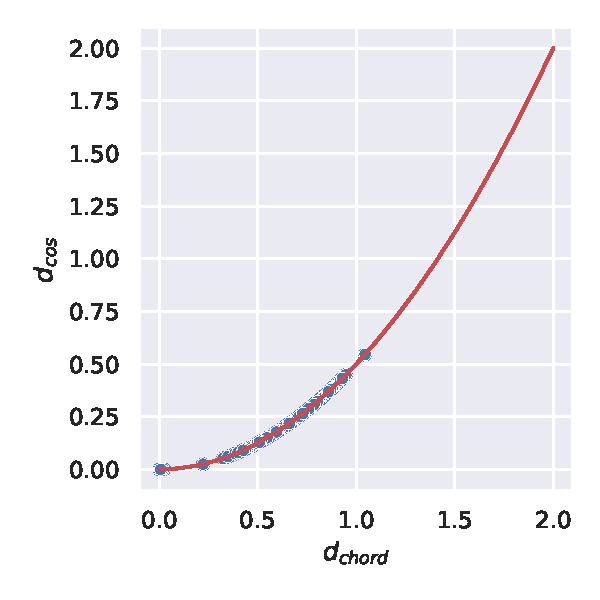
\includegraphics[width=\textwidth]{UMAP/Difference_Distance_Calculation.pdf}
    \end{subfigure}
    %\end{adjustbox}
    \caption[Cosine Distance Approximation with L2 Normalisation]{\textbf{Cosine Distance Approximation with L2 Normalisation.} .}
    \label{fig:Normalisation_Methods}
\end{figure}

The parameters used in this project with settings varying from the default are listed below. All available settings can be fount in the \href{https://scikit-learn.org/stable/modules/generated/sklearn.preprocessing.normalize.html}{API}

\begin{leftbar}
    \textbf{sklearn.preprocessing.normalize}
    \begin{nstabbing}
        \qquad\qquad\qquad\qquad\qquad\quad\=\kill
        
        X \> \\
        
        norm \> (default: ’l2’)
        
    \end{nstabbing}
\end{leftbar}